\documentclass[a4paper,11pt]{article}

% --- Geometry & Spacing (brief: 2--2.5cm margins, 1.1x line spacing) ---
\usepackage[margin=2.2cm]{geometry}
\usepackage{setspace}
\setstretch{1.1}

% --- Fonts (brief: Helvetica / Arial family, 11pt body) ---
\usepackage[T1]{fontenc}
\usepackage{helvet}
\renewcommand{\familydefault}{\sfdefault}

% --- Prevent orphan headings / widows ---
\widowpenalty=10000
\clubpenalty=10000
\raggedbottom

% --- Graphics & Wireframing ---
\usepackage{tikz}
\usetikzlibrary{shapes,arrows.meta,positioning,calc,fit}
\usepackage{graphicx}
\usepackage{pdfpages}

% --- Tables & Lists ---
\usepackage{booktabs}
\usepackage{longtable}
\usepackage{enumitem}

% --- Headers & Page Numbers (brief: pages must be numbered) ---
\usepackage{fancyhdr}
\pagestyle{fancy}
\fancyhf{}
\fancyfoot[C]{\thepage}
\renewcommand{\headrulewidth}{0pt}

% --- Hyperlinks & PDF bookmarks ---
\usepackage[hidelinks,bookmarks=true,pdfusetitle]{hyperref}

% --- Referencing: Harvard style (brief requirement) ---
\usepackage[style=authoryear,backend=biber]{biblatex}
\addbibresource{references.bib}

% ============================================================
\begin{document}

% --- Cover Page (brief: name, module code & year, ToC) ---
\begin{titlepage}
    \centering
    \vspace*{3cm}
    {\LARGE\bfseries StudyBuddy\par}
    \vspace{0.4cm}
    {\Large CW1 Supporting Materials\par}
    \vspace{1.5cm}
    {\large IN3065 User-Centred System Design 2025--2026\par}
    \vspace{1cm}
    {\large Anker Rasmussen \\230022888\par}
    \vfill
    \newpage
    \tableofcontents
    \vspace{2cm}
\end{titlepage}

% ============================================================
% PRESENTATION SLIDES (brief: A4, max 2 slides per page)
% ============================================================
\newpage
\section{Presentation Slide Deck}

\includepdf[pages=-,nup=1x2,frame=true,landscape=false,pagecommand={}]{../Presentation.pdf}

% ============================================================
% RESEARCH MATERIALS
% ============================================================
\newpage
\section{Research Materials}
The main goal when creating these interviews is to understand the existing study flow occurring for the average student.
I'd like to target students (particularly those who are preparing for exams and studying across the year). Flow will be
prescreening questionnaire, if they have the right profile (will capture emails), send information sheet. Will schedule a 
time for the actual interview, then complete the informed consent form during the interview, where they can ask questions.
After this, I'll follow my interview script, with deviation depending on their answers (semi-structured). 


\subsection{Prescreening Questionnaire}
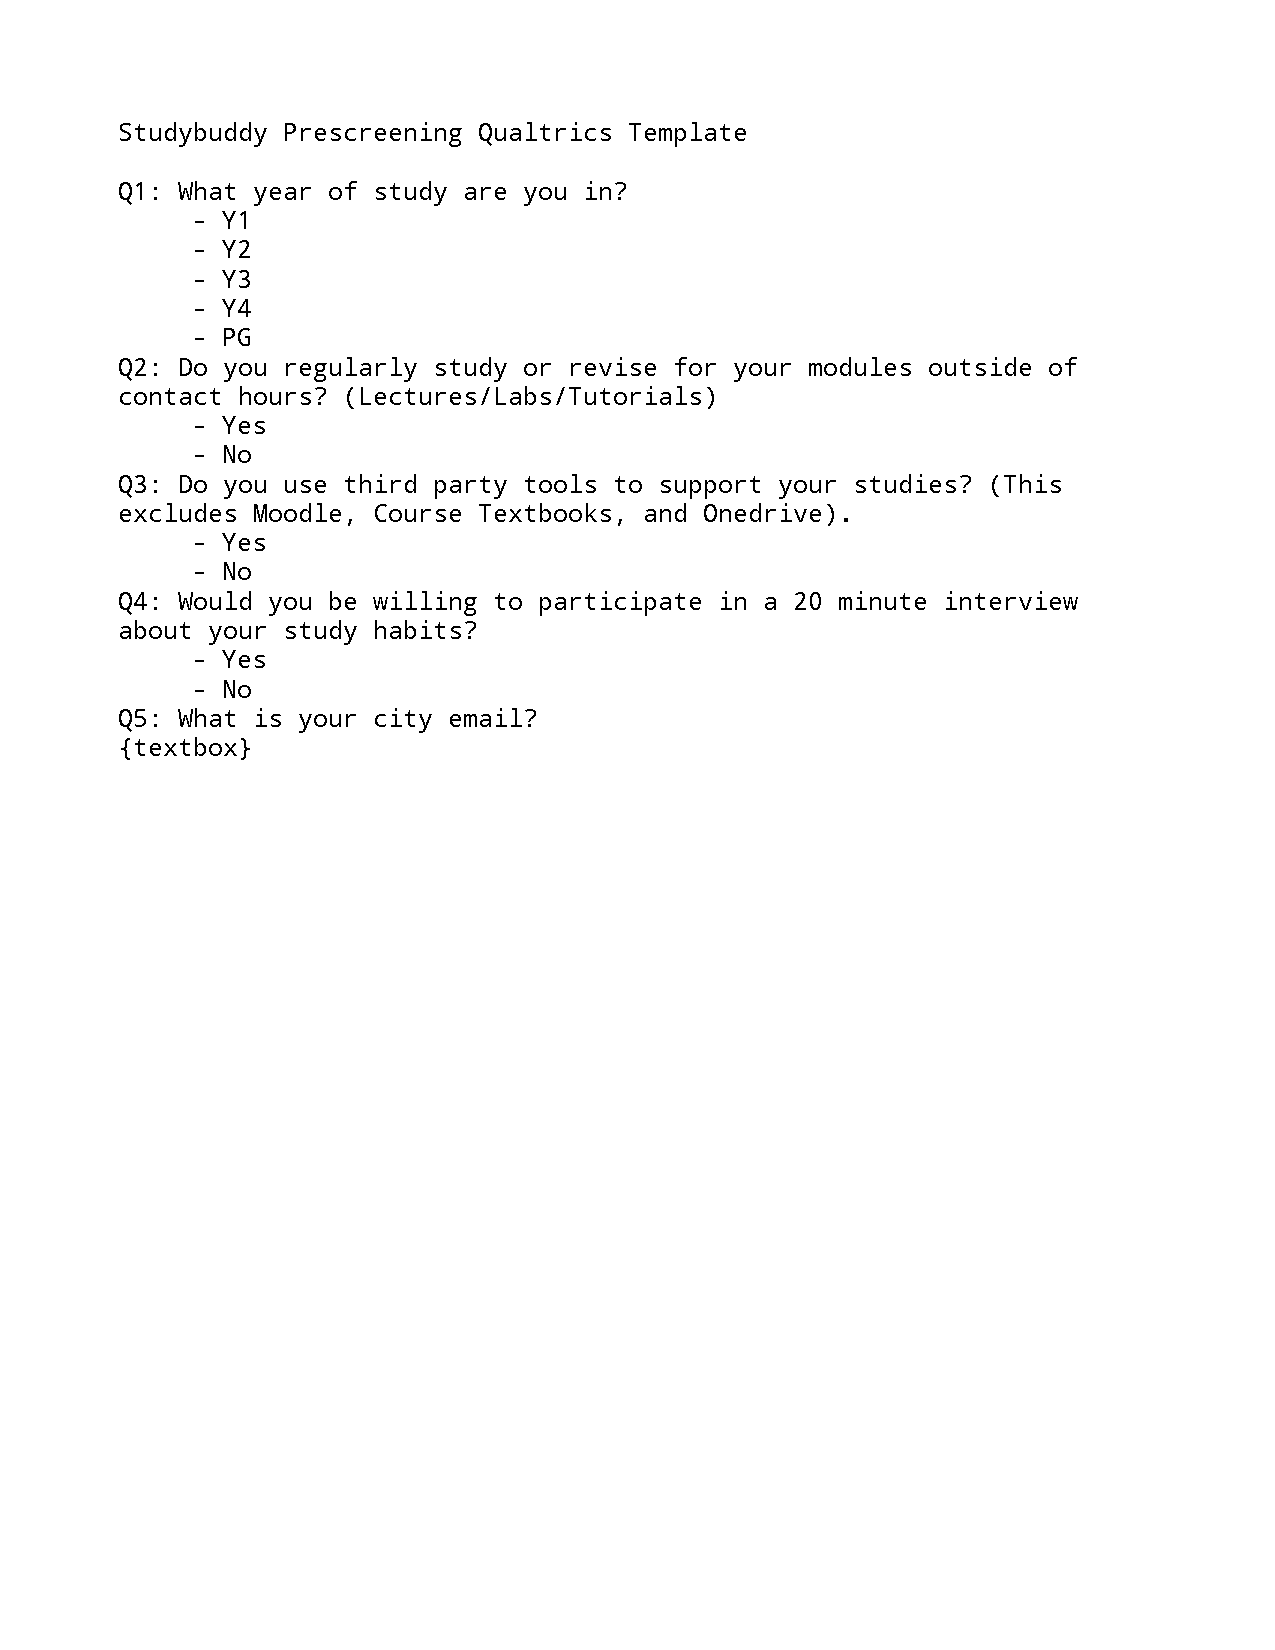
\includepdf[pages=-,pagecommand={}]{../Qualtrics.pdf}

\subsection{Participant Information Sheet}

\includepdf[pages=-,pagecommand={}]{../UCSD-CW-Ethics-Participant Information Sheet template-v1.2.pdf}


\subsection{Informed Consent Form Template}
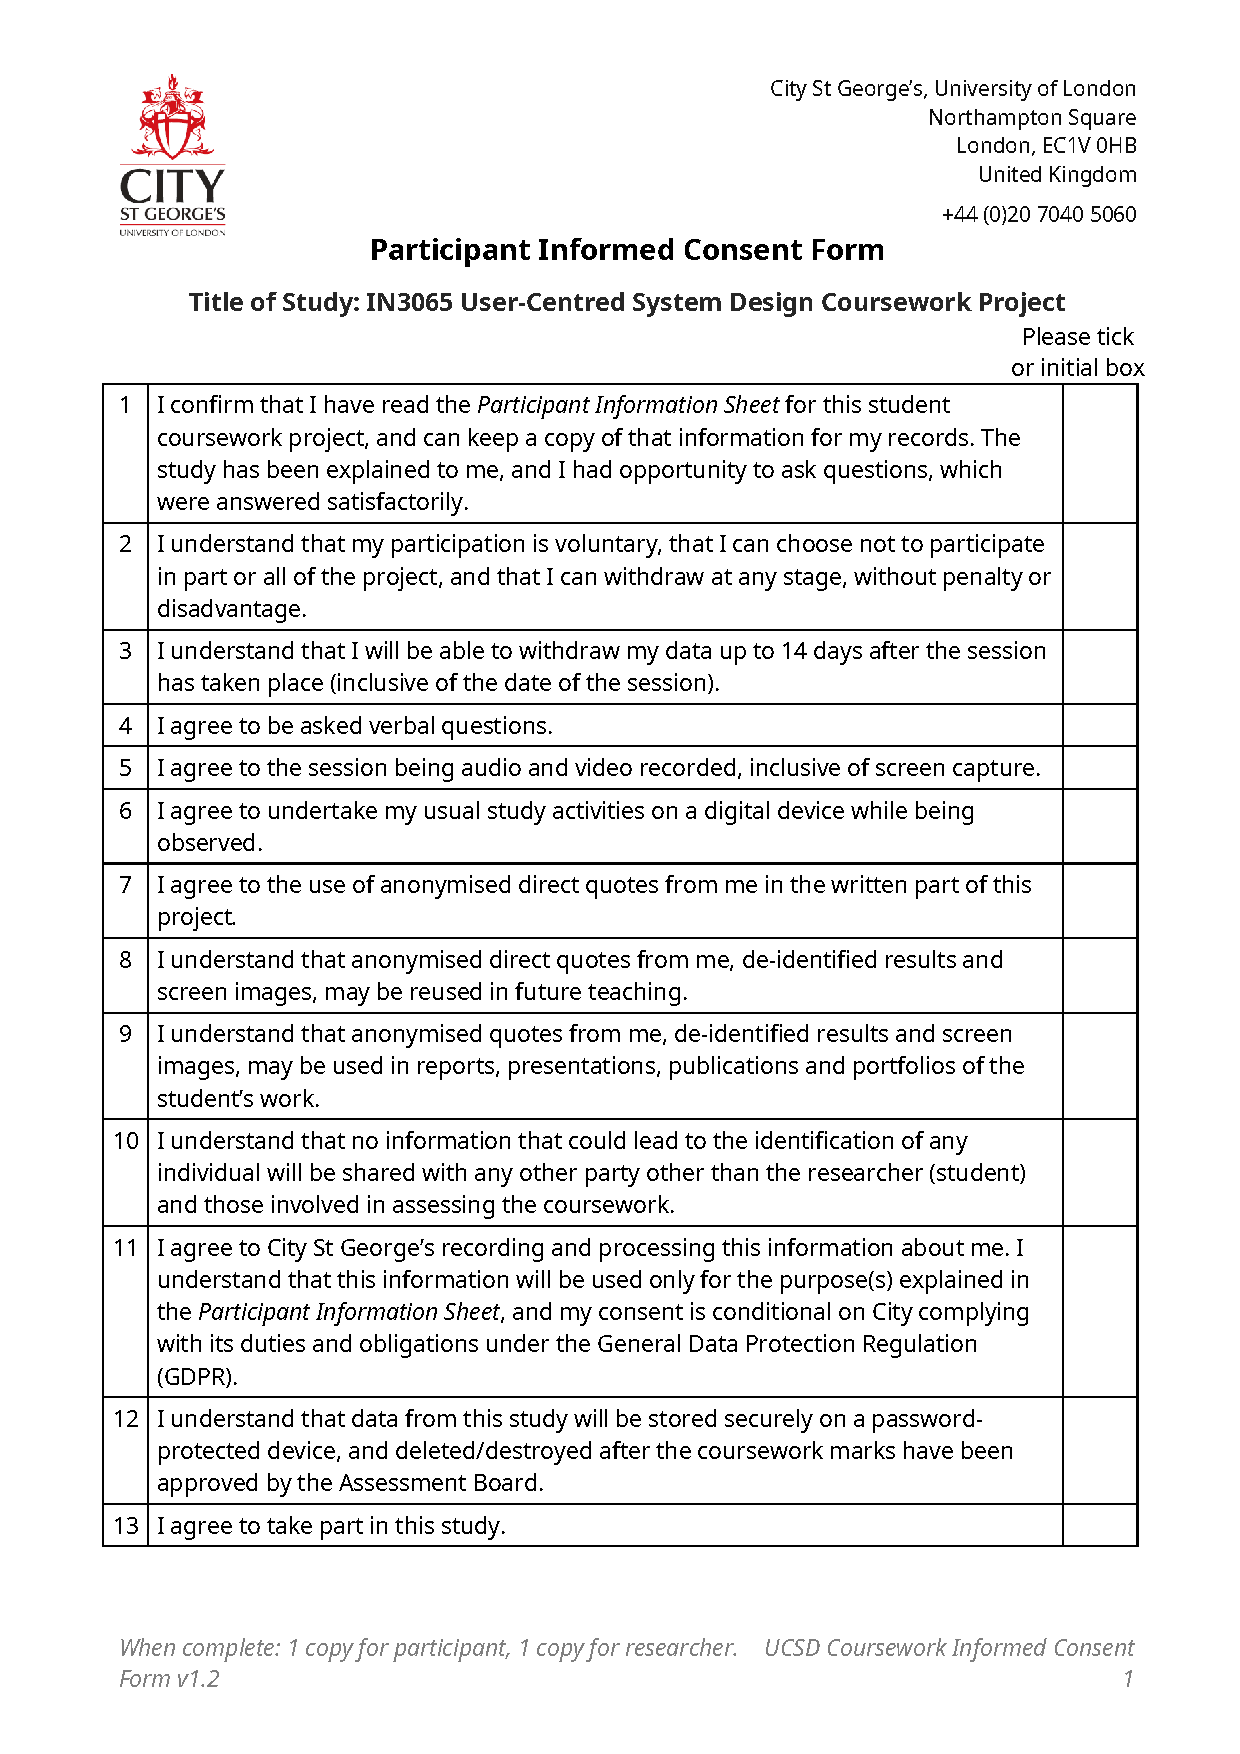
\includepdf[pages=-,pagecommand={}]{../UCSD-CW-Ethics-Informed Consent Form template-v1.2.pdf}

\newpage
\subsection{Interview Guide/Script}
This is a semi-structured interview with the goal of evolving and adapting with the interviewee's experiences to get the richest content.
Big overarching topics to try to get content related from each interview.
\subsubsection*{Interview Goals}
% What do you want to learn from these interviews?
% e.g. Understand how students currently plan and manage study sessions...
Figure out how students are currently studying with regard to their current modules, exams, quizzes, and extracurriculars.
Understand exactly how they study, if it differs between different types of modules. Understand current 
flows, what are critically missing from existing solutions, what they wish they could have, friction, and things other solutions do well.
I'd also like to understand the environment normally studied in (home, library, with friends, third spaces).


\subsubsection*{Topic Headings}
\begin{enumerate}
    \item Planning study time.
    \item Study environment.
    \item Study session itself.
\end{enumerate}

\subsubsection*{Introduction Script}
% Introduce yourself, explain the purpose of the interview, name the project
% (StudyBuddy), set expectations (duration, recording, right to decline), etc.
Hi, good \{time of day\}, as I'm sure you read in the brief, you know I'm here to interview you. This should take roughly 20 minutes, depending 
on how much we have to talk to one another, but don't worry about overrunning. It's better to talk too much than too little. I'm gonna be doing some requirements gathering
about a new application that will help you study (hopefully). You've signed the consent form but it's entirely ok if there's a question that I ask that you 
choose not to answer, and I will be recording this, which you can also request to have deleted/not have yourself participate in this. I'm also going to be taking
simple notes that help me maintain context through this interview, but this will also be transcribed (so I don't have to type everything!) So! Now that I've completed 
this formality, we can get started. 
\subsubsection*{Warmup Questions}
\begin{itemize}
    \item We're gonna start easy, what modules do you have this semester? (notes for this for callbacks!)
    \begin{itemize}
        \item How would you rank them in difficulty?
        \item What do you do in \{most-least difficult\} modules? (note: looking for type of work done, maths heavy, physics heavy, essay heavy, maybe just a lot of reading?)
    \end{itemize}
    \item Is moodle integral to your study materials/planning? (notes for this for callbacks!)
\end{itemize}

\subsubsection*{Primary Questions}

\paragraph{Topic 1: Planning the study time}
\begin{itemize}
    \item Do you structure your day for studying? (easy follow ups)
    \begin{itemize}
        \item \textbf{If yes:}
        \begin{itemize}
            \item How do you prioritize your modules?
            \item Followup: Do you give more time to difficult modules? 
            \item Followup: A different strategy per module?
        \end{itemize}
        \item \textbf{If no:}
        \begin{itemize}
            \item Why not?
            \item followup: Do you want to make your day more structured? (think calendar telling you study \{callback to module\} for xyz minutes).
        \end{itemize}
    \end{itemize}
    \item Do you have your study materials easily accessible when you study? (use Moodle as lynchpin to drive further questions)
    \begin{itemize}
        \item \textbf{If yes:}
        \begin{itemize}
            \item Do you have a sorted system when it comes to studying?
            \item How do you arrange your study materials?
        \end{itemize}
        \item \textbf{If no:}
        \begin{itemize}
            \item How do you feel about Moodle's offerings when it comes to structuring study material?
            \item Do you collate the material on your local disk? (ssd/hdd.)
        \end{itemize}
    \end{itemize}
    \item Do you use any applications/webapps to help you study? (examples: Notion, quizlet, anki, etc..)
    \begin{itemize}
        \item How effective are these tools?
    \end{itemize}
\end{itemize}

\textbf{\\Intermezzo topic switch:} \\So! We've discussed a little about your structure \textit{for} studying, but now we're gonna talk about the environment.
\paragraph{Topic 2: Study environment}
\begin{itemize}
    \item In your opinion, what makes a good (or bad!) study space?
    \begin{itemize}
        \item Let's dig into it, why?
    \end{itemize}
    \item Where do you do most of your studies? (notes for this for callbacks!)
    \begin{itemize}
        \item Do you find yourself more productive in one place?
        \item What are the most important things in this space? (silence, lack of distraction, ease of access to technology\ldots?)
        \item \{If not in a public space (i.e.\ at home)\} How do you guarantee these things?
    \end{itemize}
    \item When wanting to study, is it difficult to get everything set up?
    \begin{itemize}
        \item \textbf{If yes:}
        \begin{itemize}
            \item Let's dig into it! What troubles specifically do you have?
        \end{itemize}
        \item \textbf{If no:}
        \begin{itemize}
            \item Must be organized! Do you have a ``ritual'' to get the study environment into a conducive environment?
        \end{itemize}
    \end{itemize}
    \item Would you say you get distracted often in \{place\}?
    \begin{itemize}
        \item Is there something you do to remedy this? (noise cancelling earphones, moving, studying at weird hours)
    \end{itemize}
\end{itemize}
\textbf{\\Intermezzo topic switch \#2:}\\Let's get to the final section; your actual study session!
\paragraph{Topic 3: The actual study session}% Name your topic
\begin{itemize}
    \item When you do your studies, do you work alone or with others? (many different routes; alone, others, mixed)
    \begin{itemize}
        \item Let's talk a little about your preferred way to study. What advantages does \{preferred way\} have over others?
        \item How often do you get to study in an ideal environment? <-followups strongly recommended!
    \end{itemize}
    \item Do you prefer to snack while doing studies?
    \begin{itemize}
        \item Does this factor into your location choice whatsoever?
        \item Has this ever negatively impacted your studies?
    \end{itemize}
    \item (note: only if they do group studies) When you study with others, how do you coordinate?
    \item How do you track what you did in the session?
\end{itemize}

\subsubsection*{Walkthrough / Observation}
\begin{itemize}
    \item Let's walk through a typical study session! You'll be doing this on your device, so if you wouldn't mind sharing your screen.
    \begin{itemize}
        \item Lay the scene out for me.
        \item How did you decide where to study?
        \item How did you decide when to set up your study time?
        \item Probe: what factors influenced this?
        \item What topic did you choose to study?
        \item Probe: Why this one? (callback: Maybe one of the tougher topics)
        \item Did you study in a group this session?
        \item Probe: If yes; how did you coordinate? If no, why not?
        \item What study tools did you use (examples: moodle, quizlet etc..)
        \item Probe: Why did you use tool \{a,b,c\}?
        \item Probe: Tools used, difficulties, interruptions, snacks, successful vs unsuccessful in their eyes?
        \item Probe: How successful was the session? 
        \item Followup; how do you gauge session success?
    \end{itemize}
\end{itemize}

\subsubsection*{Closing}
Thank you for your time and participation. Before we wrap this up, is there anything more you'd like to add that we haven't covered with regard to your study habits?


% ============================================================
% REFERENCES (brief: Harvard style, before appendices)
% ============================================================
\newpage
\printbibliography[heading=bibintoc]

% ============================================================
% APPENDICES (brief: each starts on new page, listed in ToC)
% ============================================================
\newpage
\appendix

\section{GenAI Usage Log}\label{app:genai}

The following table documents all use of Generative AI tools during the
preparation of CW1 materials, including prompts/inputs, outputs and uses.

\vspace{0.5em}
\noindent
\begin{longtable}{@{}p{1.8cm}p{2.8cm}p{4.5cm}p{4.5cm}@{}}
\toprule
\textbf{Date} & \textbf{Tool} & \textbf{Prompt/Input} & \textbf{Output \& Use} \\
\midrule
\endhead
2026-02-18
& Claude Opus 4.6 (Claude Code CLI)
& \texttt{Read through brief.pdf, create wireframe .tex, and attribute this
  prompt and your creation of the wireframe in the appendix of pt1 (cw1).}
& Generated the initial \LaTeX{} document skeleton for CW1 (section structure,
  package imports including TikZ, cover page, appendix layout, and this GenAI
  log).  Wireframe content will be authored manually. \\
\midrule
2026-02-18
& Claude Opus 4.6 (Claude Code CLI)
& \texttt{no; don't do wireframes, just create the sections.\ ill make the
  wireframes myself (just import the tikz package).\ [\ldots] pt1 is pt1.\
  create a .bib too (add this prompt to the appendix).}
& Separated wireframes into standalone \texttt{wireframe.tex}, created
  \texttt{references.bib}, removed wireframe appendix from pt1.tex, and added
  this log entry. \\
\midrule
2026-02-18
& Claude Opus 4.6 (Claude Code CLI)
& \texttt{I have latex workshop.\ make sure the format is correct (as specified
  in brief.pdf).\ (also add this prompt to the appendix).}
& Revised pt1.tex formatting to match brief requirements (margins, spacing,
  orphan prevention, longtable for GenAI log, \texttt{bibintoc} for references
  in ToC, appendix labelling).  Added this log entry. \\
\midrule
2026-02-18
& Claude Opus 4.6 (Claude Code CLI)
& \texttt{add a hook to claude where you have to attribute prompts and usage in
  the appendix for this repo.\ (also add this prompt to the appendix haha).}
& Created \texttt{CLAUDE.md} in the repo root with a standing instruction to
  always log GenAI usage to the appendix of the relevant coursework \texttt{.tex}
  file.  Added this log entry. \\
\midrule
2026-03-02
& Claude Opus 4.6 (Claude Code CLI)
& \texttt{Can you make me a quick LaTeX template based on my tutorial template
  for me to fill out in the part-1 then document the AI usage in the appendix?}
& Generated a blank interview guide template in the Interview Guide/Script
  subsection of pt1.tex, structured after the tutorial 3 handout format
  (goals, topic headings, intro script, warmup, primary questions with
  branching follow-ups, walkthrough/observation section, closing).
  All question content left blank for the student to fill in.
  Added this log entry. \\
\midrule
2026-03-07
& Claude Opus 4.6 (Claude Code CLI)
& \texttt{Hey, put in the .pdfs where they should be within the .tex file so I
  can submit it.}
& Added \texttt{pdfpages} package and \texttt{\textbackslash includepdf}
  commands to embed Presentation.pdf (2-up per page in the Slide Deck section),
  Participant Information Sheet PDF, and Informed Consent Form PDF into their
  respective sections of pt1.tex.  Added this log entry. \\
\midrule
2026-03-07
& Claude Opus 4.6 (Claude Code CLI)
& \texttt{Do one pass over my .tex, fix typos and grammatical errors.}
& Fixed 6 typos/grammar issues: ``regards to.their'' $\to$ ``regard to their'',
  ``requirement gathering'' $\to$ ``requirements gathering'',
  missing space after colon in Topic~2 heading,
  missing closing quote on ``ritual'',
  ``envrionment'' $\to$ ``environment'',
  ``Intemerzzo'' $\to$ ``Intermezzo'',
  ``unsuccesful'' $\to$ ``unsuccessful''.
  Added this log entry. \\
\midrule
2026-03-07
& Claude Opus 4.6 (Claude Code CLI)
& \texttt{Oh.\ also add my Qualtrics pdf (it's for my prescreening questionnaire).}
& Added a ``Prescreening Questionnaire'' subsection to Research Materials
  with \texttt{\textbackslash includepdf} embedding \texttt{Qualtrics.pdf}.
  Added this log entry. \\
\bottomrule
\end{longtable}

\end{document}
